\documentclass{marine_2015}
     
\usepackage{graphicx}
\usepackage{amsmath}
\usepackage{amsfonts}
\usepackage{amssymb}

\newcommand{\Amat}{\ensuremath{\mathbb{A}}}
\newcommand{\Bmat}{\ensuremath{\mathbb{B}}}
\newcommand{\bvec}{\ensuremath{\mathbf{b}}}
\newcommand{\uvec}{\ensuremath{\mathbf{u}}}
\newcommand{\RM}{\ensuremath{RM}}
\newcommand{\inner}[2]{\ensuremath{\left(#1, #2\right)}}
\newcommand{\tuple}[2]{\ensuremath{\left[#1, #2\right]}}

\newcommand{\ainner}[2]{\ensuremath{a\left(#1, #2\right)}}
\newcommand{\binner}[2]{\ensuremath{b\left(#1, #2\right)}}
\newcommand{\Linner}[1]{\ensuremath{L\left(#1\right)}}
\newcommand{\Vh}{\ensuremath{V_{\mathbf{n}}}}
\newcommand{\Qh}{\ensuremath{Q_{\mathbf{m}}}}

\newcommand{\norm}[1]{\ensuremath{\left\|#1\right\|}}
\newcommand{\vvec}[1]{\ensuremath{\pmb{#1}}}
\newcommand{\deriv}[2]{\ensuremath{\frac{\mathrm{d}#1}{\mathrm{d}#2}}}
\newcommand{\tderiv}[2]{\ensuremath{\tfrac{\mathrm{d}#1}{\mathrm{d}#2}}}

\title{
  BEND$\left|\text{P}\right|$Y: PYTHON FRAMEWORK FOR COMPUTING BENDING OF COMPLEX PLATE-BEAM SYSTEMS
}

\author{MIKAEL MORTENSEN$^{1, 2}$ AND MIROSLAV KUCHTA$^{1}$ AND KENT-ANDRE MARDAL$^{1, 2}$ }

\heading{Mikael Mortensen, Miroslav Kuchta and Kent-Andre Mardal}

\address{$^{1}$
Department of Mathematics, Division of Mechanics, University of Oslo,\\
0316 Oslo, Norway
  \and
$^{2}$ 
Center for Biomedical Computing, Simula Research Laboratory,\\
P.O. Box 134, No-134 Lysaker, Norway
}

\keywords{biharmonic equation, Lagrange multipliers, Schur complement}

\abstract{
We present a light-weight Python module for computing small deformations of a 
single plate supported by an arbitrary number of possibly intersecting
stiffeners. We show how the problem fits into the framework of abstract 
saddle point problems and how this abstraction can be exploited for clean design 
of the code. Stability properties of the resulting linear systems for two different 
sets of basis functions, namely, the eigenfunctions of the biharmonic operator 
and specialized Legendre polynomials are discussed. 
}

\begin{document}

\section{Introduction}
% What are we solving?
In this paper we discuss Galerkin methods for finding the equilibrium state of a 
physical system formed by a loaded thin plate and several beams which are constrained 
to deform together with the plate. Denoting $k$ the number of supporting beams, 
the equilibrium state is found as the solution of a constrained minimization problem
\begin{equation}
  \label{eq:foo}
  u = \min_{v\in V} \mathcal{E}\left(v\right)\quad\text{ and }\quad u_0\circ F_r
  = u_r, r=1, 2, \cdots k,
\end{equation}
where the energy functional $\mathcal{E}$ is defined as
\[
  \mathcal{E}\left(u\right)=
    \frac{E_0}{2}\displaystyle\int_{\Omega}\Delta u_0\,\Delta u_0+
    \sum_{r=1}^k\frac{E_r}{2}\int_{\mathcal{I}}
  \deriv{^2u_r}{s^2}\deriv{^2u_r}{s^2}J_r^{-3}
  -\displaystyle\int_{\Omega}f u_0.
\]
Here $V=V_0\times V_1 \times\cdots\times V_k$ is a function space with $k+1$
components. The first component $V_0$ contains functions that map the plate
domain $\Omega$ to real numbers and is therefore the space where the plate's
vertical displacement $u_0$ is found. The remaining components in $V$ contain the 
vertical displacements of individual beams $u_r$, i.e., the scalar 
functions whose domain is the interval $\mathcal{I}$. Moreover each beam is
considered as a set $\Gamma_r=\left\{x\in\Omega, x=F_r\left(s\right), s\in\mathcal{I}\right\}$
defined by an invertible mapping $F_r$ with Jacobian $J_r$. Note that for straight 
beams which are in focus of the presented work the Jacobian is simply the length of
the beam divided by the length of the interval. The mapping $F_r$ is in addition 
required to satisfy the conditions $F_r\left(s_0\right), F_r\left(s_1\right)\in\partial\Omega$ 
for $s_0, s_1$ the endpoints of $\mathcal{I}$. No beam is thus allowed to end inside 
the plate. Finally $f$ denotes the load while $E_0, E_r, r=1,2,\cdots k$ are 
constant parameters which, following the Kirchhoff-Love and Euler-Bernoulli
hypothesis (e.g. \cite{reddy}), depend on the material and geometry.

Introducing $k$ Lagrange multipliers $\lambda_k\in Q_k$, where the functions in 
$Q_k$ map the interval $\mathcal{I}$ to scalars, the constrained problem 
(\ref{eq:foo}) can be equivalently written as a search for extrema of the Lagrangian
$\mathcal{L}$,
\begin{equation}
  \label{eq:bar}
\mathcal{L}\left(u, \lambda\right) = \mathcal{E}\left(u\right) +
  \sum_{r=1}^k\int_{\mathcal{I}}\left(u_0\cdot F_r - u_r\right)\lambda_r J_r.
\end{equation}
The space $Q$ and function $\lambda\in Q$ are defined analogically as in (\ref{eq:foo}).
We note that the unconstrained problem (\ref{eq:bar}) is solvable only for
suitable pair of spaces $V, Q$ for which the requirements of the
Babu\v{s}ka-Brezzi\cite{babuska, brezzi} theory are satisfied.

% It can be solved with FEM but simple geometry ... global functions, spectral
% Galerkin
For a complex domain $\Omega$ the finite element method is arguably the most 
suitable method to solve the problem (\ref{eq:bar}). If, on the other hand, the
domain is simple, the Galerkin method with globally supported basis functions
can be applied. Note that the finite element method is an instance of the Galerkin 
method with test spaces spanned by the functions with local support. Regardless
of the basis functions employed, the stable discretization of (\ref{eq:bar})
requires that the Babu\v{s}ka-Brezzi conditions be satisfied by the constructed
finite dimensional spaces. We remark that in addition to stability
considerations the finite element discretization of problem is also complicated
by presence of the biharmonic operator which requires techniques for fourth order 
problems (see e.g. \cite{brenner}). The approximations of $V$ must be constructed 
from $C^1$ continuous elements, e.g. Argyris element \cite{argyris}, or non-conforming 
elements, e.g. Morley element\cite{morley}. Alternatively, discontinuous elements with 
suitable stabilization \cite{brenner_ip} can be used. 

Here we shall consider the plate as a simply connected rectangular domain and as
such focus on Galerkin methods with test functions having the global support.
Further, the two selected basis are designed for the fourth order problems and thus 
only the Babu\v{s}ka-Brezzi theory needs to be considered to derive a stable
discretization of problem (\ref{eq:bar}). The methods are discussed within a
framework for abstract saddle point problems reviewed in Section
\ref{sec:abstract}. The framework serves to identify the few common
elements(matrices) that are required to easily introduce Galerkin discretizations of
(\ref{eq:bar}) based on any set of basis functions. Properties of the two sets of
basis functions considered in this paper are then compared in Section \ref{sec:basis}.
Finally in Section \ref{sec:lbb} the inf-sup condition for the two proposed
disretizations is discussed.

\section{Abstract framework for saddle point problems}
\label{sec:abstract}
% conditions for extrema
The necessary conditions for the extreme point of the Lagrangian $\mathcal{L}$
from (\ref{eq:bar}) define $2k+1$ equations to be satisfied by the $2k+1$
unknowns $\left(u, \lambda\right)\in V\times Q$. These equations read
\[
  \begin{aligned}
    \label{eq:system}
    E_0\displaystyle\int_{\Omega}\Delta u_0\,\Delta v_0-
    \sum_{r=1}^k\int_{\mathcal{I}}v_0\lambda_r J_r &=\displaystyle\int_{\Omega}f
    v_0\quad\forall v_0\in V_0,& \\
    E_r\displaystyle\int_{\mathcal{I}}
    \deriv{^2u_r}{s^2}\deriv{^2v_r}{s^2}J_r^{-3} +
  \int_{\mathcal{I}} u_r \lambda_r J_r &= 0\quad\forall v_r\in V_r, r=1,
    2\cdots, k,&\\
  \int_{\mathcal{I}}\left(u_r-u_0\right)\mu_r J_r &= 0\quad\forall \mu_r\in Q_r,
    r=1, 2\cdots, k&.\\
  \end{aligned}
\]
To apply the Babu\v{s}ka-Brezzi theory of abstract saddle point problems to (\ref{eq:system})
the system is rewritten in terms of bilinear forms $a:V\times V\mapsto \mathbb{R}$, $b:Q\times V\mapsto \mathbb{R}$
and a linear form $L:V\mapsto R$. Here 
$\ainner{u}{v}=\sum_{r=0}^{k}\ainner{u_r}{v_r}_r$ where




% how the problem fits saddle
% Galerkin and how A, B are formed for r. The elements that are needed for
% efficiency: mass, stiffness, bending, (fast inner product). Probably mention sparsity
% Eigenvalue problem for LBB.





Let $\mathcal{I}$ denote a nonempty interval. As we are in the following
interested in domains that have a Cartesian product structure we consider without
loss of generality $\Omega=\mathcal{I}\times\mathcal{I}$. We shall refer to this
domain as \textit{plate}. Further let $w_i, i=1, 2,\cdots, k$ be a set of curves 
$w_i=\left\{\vec{x}\in\Omega, \vec{x}=\vec{F}_i\left(s\right),
s\in\mathcal{I}\right\}$, where $\vec{F_i}$ is a smooth invertible mapping with
Jacobian $J_i>0$ that additionally satisfies $\vec{F}_i\left(s_0\right),
\vec{F}_i\left(s_1\right)\in\partial\Omega$ and
$\vec{F}_i\left(s_0\right) \neq \vec{F}_i\left(s_1\right)$ for $s_0, s_1$ the
endpoints of interval $\mathcal{I}$. These curves, and occasionally the
respected mappings are referred to as \textit{beams}. In this paper we are for the
most part concerned with straight/linear beams, that is, we consider mappings
$\vec{F}_i\left(s\right)=\vec{P}_i\tfrac{s_1-s}{s_1-s_0}+\vec{Q}_i\tfrac{s_0-s}{s_0-s_1}$
determined by pairs of mutually distinct points $\vec{P}_i, \vec{Q}_i$ which
are located on the boundary of the plate. Note that in this case
$J_i=\tfrac{\left|\vec{P}_i-\vec{Q}_i\right|}{2}$.
% you do linear so absorb jacobian into material!!! KISS
%
%
%
With these assumptions on geometry we let $V, \hat{V}_i, i=1, 2, \cdots, k$ denote
spaces of functions that map respectively the plate and the beams to real
numbers. By invertibility of $\vec{F}_i$ each function space $\hat{V}_i$ can be
associated with a function space that $V_{i}$ that maps the reference interval
$\mathcal{I}$ to real numbers. Indeed for $v\in V_i$ function
$\hat{v}=v\circ\vec{F}_i$ belongs to $\hat{V}_i$.

Let $u\in V, u_i\in V_i, i=1, 2, \cdots, k$ and consider the problem of
minimizing the Lagrangian
\[
  \mathcal{L}\left(u, u_1, u_2, \cdots, u_k\right)=
  \frac{E}{2}\displaystyle\int_{\Omega}\Delta u\,\Delta u+
  \sum_i\frac{E_i}{2}\int_{\mathcal{I}}
  \deriv{^2u_i}{s^2}\deriv{^2u_i}{s^2}J_i^{-3}
  -\displaystyle\int_{\Omega}f u
\]
subjected to $k$ constraints
$T(u)=u_i$, here $T(u)$ is a short hand for the composition of trace and the
pullback inverse.\textit{explain the constraint, trace, Sobolev?}.
We build the constraint into the Lagrangian. To this end consider spaces $Q_i$
and functions (Lagrange multipliers) $\lambda_i\in Q_i$. Moreover let
$Q=Q_0\times Q_1\times\cdots\times Q_k$ and $\vvec{\lambda}\in
Q,\vvec{\lambda}_i=\lambda_i$ and a problem
\[
  \mathcal{L}\left(u, u_1, u_2, \cdots, u_k;\vvec{\lambda}\right)=
   \frac{E}{2}\displaystyle\int_{\Omega}\Delta u\,\Delta u+
  \sum_i\frac{E_i}{2}\int_{\mathcal{I}}
  \deriv{^2u_i}{s^2}\deriv{^2u_i}{s^2}J_i^{-3}
  -\displaystyle\int_{\Omega}f u - \sum_i\int_{\mathcal{I}}\left(u-u_i\right)\lambda_i J_i
\]
The necessary condition for extrema are then
Under additional regularity we can make Euler Lagrange equations
\[
  \begin{aligned}
    E\Delta^2u &= f\quad\text{ in }\Omega\\
    E_i\deriv{^4 u_i}{s^4} &= 0\quad\text{ on }\mathcal{I}\\
    u &= u_i\quad\text{ on }\mathcal{I}\\
  \end{aligned}
\]
subjected to boundary conditions $u=0, \partial_nu=0$ and $u_i=0, \tderiv{u_i}{s}=0$
$u=0, \Delta u=0$ and $u_i=0, \tderiv{^2u_i}{s^2}=0$. \textit{What are these called?}
Abstract saddle $V:=V\times V_1, \times V_2, \cdots, \times V_k$,
$V\ni\vvec{u}=\left(u, u_1, u_2, \cdots, u_k\right)$ and define bilinear form
$a:V\times V\mapsto\mathbb{R}$ as
\[
  \ainner{\vvec{u}}{\vvec{v}} = 
  E\displaystyle\int_{\Omega}\Delta u\,\Delta+
  \sum_iE_i\displaystyle\int_{\mathcal{I}} \deriv{^2u_i}{s^2}\deriv{^2v_i}{s^2}J_i^3
\]
$b:V\times Q\mapsto\mathbb{R}$ as
\[
  \binner{\vvec{v}}{\vvec{\lambda}} = 
  \int_{\mathcal{I}}\left(v_i-v\right)\lambda_i J_i
\]
Finally linear form
$L:V\mapsto\mathbb{R}$ as
\[
  \displaystyle\int_{\Omega}f v
\]
%FIXME it is much better to use V_0 and then V...
% Saddle
Then the problem becomes simply: Find $\vvec{u}\in V, \vvec{\lambda}\in Q$ such
that $\ainner{u}{v}+\binner{v}{\lambda}+\binner{u}{\mu}=\Linner{v}$ for all 
$\vvec{v}\in V, \vvec{\mu}\in Q$. You have babuska theory that gives you
continuous existence. Don't go there... Discrete mention Stokes taylor hood, or
the compatibility condition from spectral.
% Galerkin
The finite dimensional approximation of $V$ is $\Vh$. Here $\mathbf{n}$ is a
multiindex of length $k+1$ and $\mathbf{n}_i, i=0, 1,\cdots, k$ denotes dimension
of the $i$-th component of $\Vh$ which is spanned by functions $\phi^i_j,
i=1,2,\cdots\mathbf{n}_i$. Note that $\phi^0_j$ are defined over $\Omega$ while
the rest have the reference interval as their domain. Similarly, we denote $\Qh$ 
the finite dimensional approximation of $Q$ is . Here $\mathbf{m}$ is a multiindex
of length $k$ and $\mathbf{m}_i, i=1, 2, \cdots, k$ denotes dimension of the 
$i$-th component of $\Qh$ spanned by functions $\psi^i_j, j=1,
2\cdots,\mathbf{m}_i$.
% Matrices
Let $n, m$ be respectively the sizes of multiindices $\mathbf{n}, \mathbf{m}$.
The abstract saddle point problem considered on the discerete subspaces
translates into the linear system: Find $\mathbf{U}\in\mathbb{R}^n,
\mathbf{P}\in\mathbb{R}^m$ such that
\[
    \begin{bmatrix}
      \mathbb{A} & \mathbb{B} \\
      \mathbb{B}^{\text{T}} & 0
    \end{bmatrix}
    \,
    \begin{bmatrix}
      \mathbf{U} \\
      \mathbf{P}
    \end{bmatrix}
    =
    \begin{bmatrix}
      \mathbf{b}\\
      0
    \end{bmatrix}.
\]
$\mathbf{b}\in\mathbb{R}^n$ has most entries zero except the first $\mathbf{n}_0$
entries which take the value $\inner{\phi^0_j}{f}$. The matrix
$\Amat\in\mathbb{R}^{n\times n}$ is block diagonal consisting of $k+1$
submatrices
\[
    \mathbb{A}=
    \begin{bmatrix}
      \mathbb{A}^0  &   &  &\\
                    & \mathbb{A}^1 &  &\\
                    &   &   \ddots    & \\
                    &   &   & \mathbb{A}^k\\
    \end{bmatrix}
\]
with $\mathbb{A}^0_{i, j}=E\inner{\Delta \phi^0_i}{\Delta\phi^0_j}$ and
$\mathbb{A}^r_{i, j}=E_r\displaystyle\int_{\mathcal{I}}
\deriv{^2\phi^r_i}{s^2}\deriv{^2\phi^r_j}{s^2}J_r^3$. Matrix
$\Bmat\in\mathbb{R}^{n\times m}$
\[
    \mathbb{B}=
    \begin{bmatrix}
      \mathbb{C}^1 & \mathbb{C}^2 & \cdots & \cdots & \mathbb{C}^k\\
      \mathbb{M}^1   &        0       & \cdots & \cdots &        0      \\
           0         & \mathbb{M}^2   &    0   & \cdots &   \vdots      \\
         \vdots      &       0        & \ddots & \ddots &   \vdots      \\
         \vdots      &     \vdots      & \ddots & \ddots &       0      \\
      0         &  \cdots        & \cdots & 0      &   \mathbb{M}^k     \\
    \end{bmatrix}
\]
where $\mathbb{C}^r_{ij}=\int_{\mathcal{I}}\phi^0_j\psi^r_i$ and
$\mathbb{M}^r_{ij}=\int_{\mathcal{I}}\phi^r_j\psi^r_i$, so the latter defines
a mass matrix between spaces.
Eigenvalue problems for wellposedness/stability. Programming needs assembler
so just take into accont the multiindex to get the position and size of the
block. What are blocks: we have mass matrix and the 1d 2d bending matrices.
Simplifies if $\phi^i=\psi^i$.

% Discussion on properties of basis. Some speedup with FFT
\section{Basis}
\label{sec:basis}
% For each basis how it is defined. How does A look, convergence properties for
% biharmonic problem(What happens if discontinuity). How does A scale. Comment
% on fast assembly
\subsection{Shen basis}
Described in shen. Legendre polynomials - we use for clamped boundary
conditions. Confirm spectral convergence in 1d and 2d. In 1d the biharmonic is
diagonal hence Ak matrices. But A0 is ... . Mass matrix is penta diagonal. How
does 2d bending matrix scale. Probably mention the tensor product. Mention
forward legendre transform.
\subsection{Eigen basis}
Consider eigenvalue problem. Find functions - spectral decomposition. Action of
Galerkin method with the basis. Convergence 1d, 2d. Matrices. Solution. If you
have time it would be really nice to solve 1d solution with rhs that has
different smoothness so that we see how it effects the rate in both cases.

\begin{table}[t!]
    \begin{center}
    \begin{tabular}{ccccc}
\hline
$n$  &  $f_0: \norm{e}_0$  & $f_1: \norm{e}_0$ & $f_2: \norm{e}_0$ & $f_3: \norm{e}_0$\\
\hline
4    & 1.0577E-04(3.61) & 9.9167E-05(3.81) &       --        & 1.4040E-04(2.46) \\
8    & 6.1251E-06(4.11) & 5.7545E-06(4.11) & 2.8982E-08(5.84)& 6.2305E-06(4.49) \\
16   & 2.9912E-07(4.36) & 2.8123E-07(4.35) & 4.1493E-10(6.13)& 3.0082E-07(4.37) \\
32   & 1.3929E-08(4.42) & 1.4545E-08(4.27) & 4.8407E-12(6.42)& 1.4161E-08(4.41) \\
64   & 6.2978E-10(4.47) & 5.9356E-10(4.61) & 5.6482E-14(6.42)& 6.5283E-10(4.44) \\
128  & 2.5395E-11(4.63) & 2.4049E-11(4.63) & 8.5939E-16(6.04)& 2.7228E-11(4.58) \\
256  & 1.1403E-12(4.48) & 1.0861E-12(4.47) & 7.0351E-16(0.29)& 1.2692E-12(4.42) \\
\hline
\hline
    \end{tabular}
    \caption{sines}
  \label{tab:sine_convergence}
  \end{center}
  \end{table}


\begin{table}[t!]
    \begin{center}
    \begin{tabular}{ccccc}
\hline
$n$  &  $f_0: \norm{e}_0$  & $f_1: \norm{e}_0$ & $f_2: \norm{e}_0$ & $f_3: \norm{e}_0$\\
\hline
4 &  3.0367E-05(2.34)& 1.1478E-05(4.11)& 7.5138E-07(8.28)& 8.7249E-05(2.65)  \\ 
6 &  9.4639E-06(2.88)& 2.0211E-06(4.28)& 1.1883E-07(4.55)& 1.1292E-05(5.04) \\
8 &  3.7833E-06(3.19)& 5.5737E-07(4.48)& 2.7564E-08(5.08)& 7.2035E-07(9.57) \\
10&  1.7737E-06(3.39)& 1.9868E-07(4.62)& 1.0879E-08(4.17)& 2.8851E-08(14.42) \\
12&  9.2954E-07(3.54)& 8.3836E-08(4.73)& 3.5788E-09(6.10)& 4.2572E-10(23.12) \\
14&  5.2899E-07(3.66)& 3.9893E-08(4.82)& 1.1724E-09(7.24)& 8.7160E-12(25.23) \\
16&  3.2080E-07(3.75)& 2.0775E-08(4.89)& 6.8783E-10(3.99)& 4.7527E-14(39.03) \\
18&  2.0463E-07(3.82)& 1.1004E-08(5.40)& 4.3562E-10(3.88)& 8.3310E-15(14.78) \\
20&  1.3602E-07(3.88)& 5.4562E-09(6.66)& 2.5669E-10(5.02)& 1.7601E-14(-7.10) \\
22&  9.3564E-08(3.93)& 3.2351E-09(5.48)& 1.5121E-10(5.55)& 2.0605E-13(-25.81)\\
24&  6.3166E-08(4.52)& 2.3836E-09(3.51)& 7.8326E-11(7.56)& 2.8589E-13(-3.76) \\
26&  4.8081E-08(3.41)& 1.9361E-09(2.60)& 4.5928E-11(6.67)& 1.0247E-12(-15.95)\\
28&  3.2319E-08(5.36)& 1.2840E-09(5.54)& 3.0818E-11(5.38)& 1.9021E-12(-8.35) \\
30&  2.0739E-08(6.43)& 9.6124E-10(4.20)& 1.7277E-11(8.39)& 2.7543E-11(-38.74)\\
\hline
    \end{tabular}
    \caption{shen}
  \label{tab:shen_convergence}
  \end{center}
  \end{table}



\begin{figure}[ht]
\centering
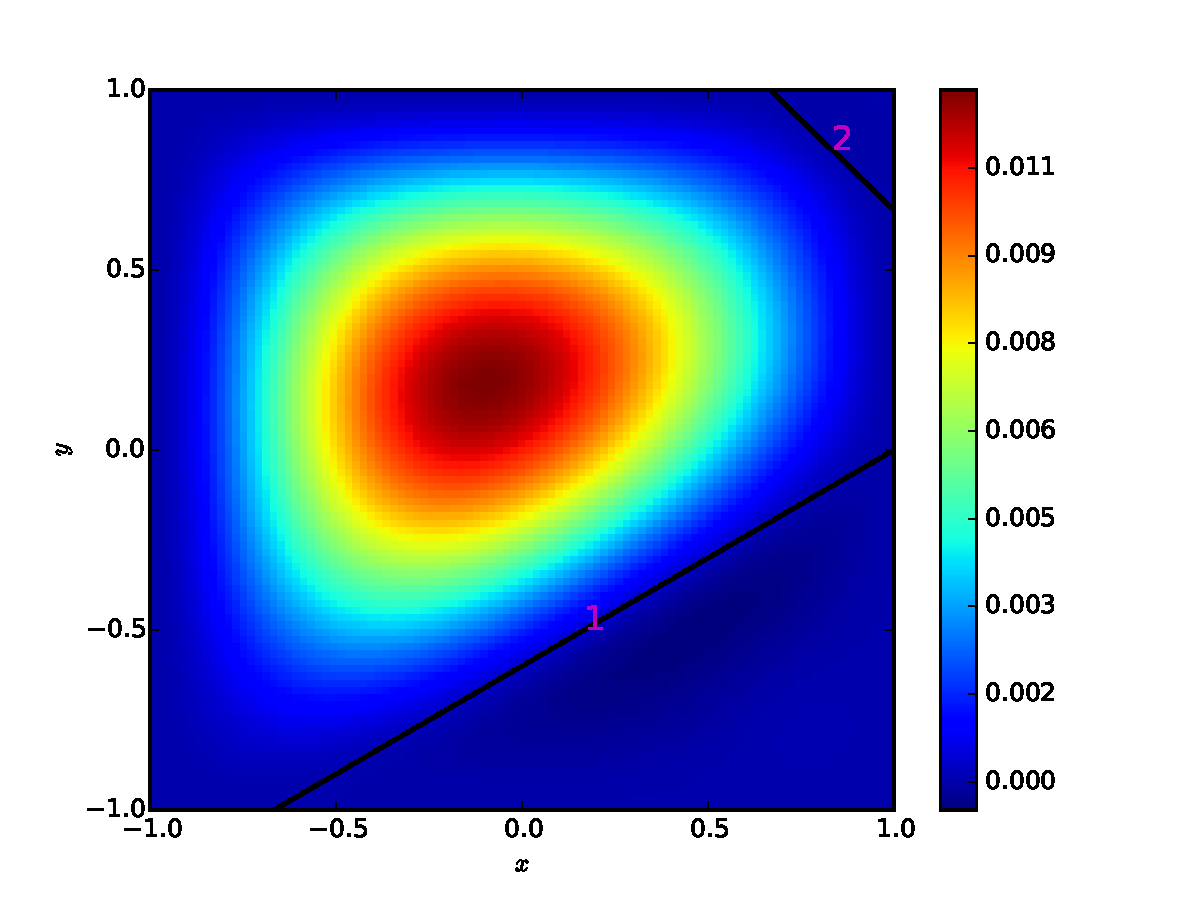
\includegraphics[width=0.45\textwidth]{img/shen_u0}
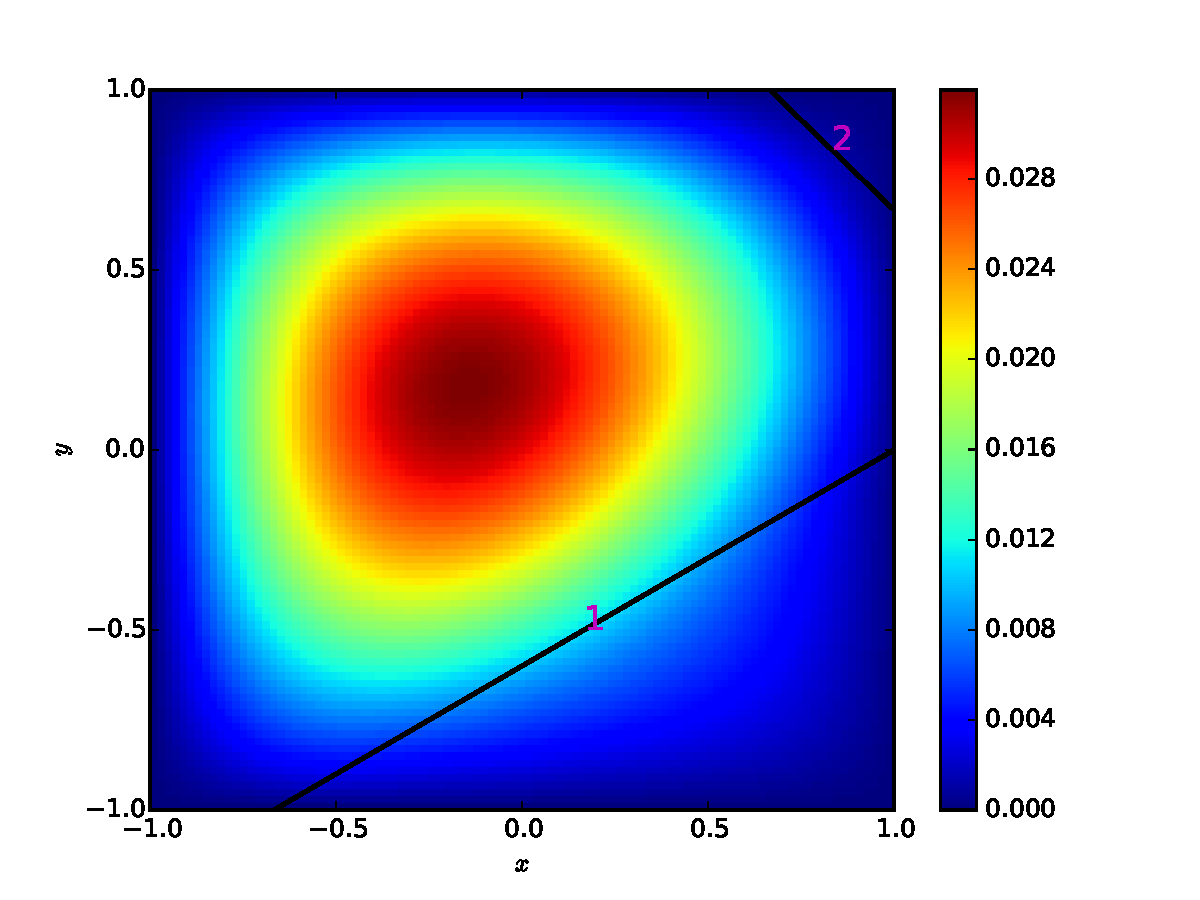
\includegraphics[width=0.45\textwidth]{img/sine_u0}\\
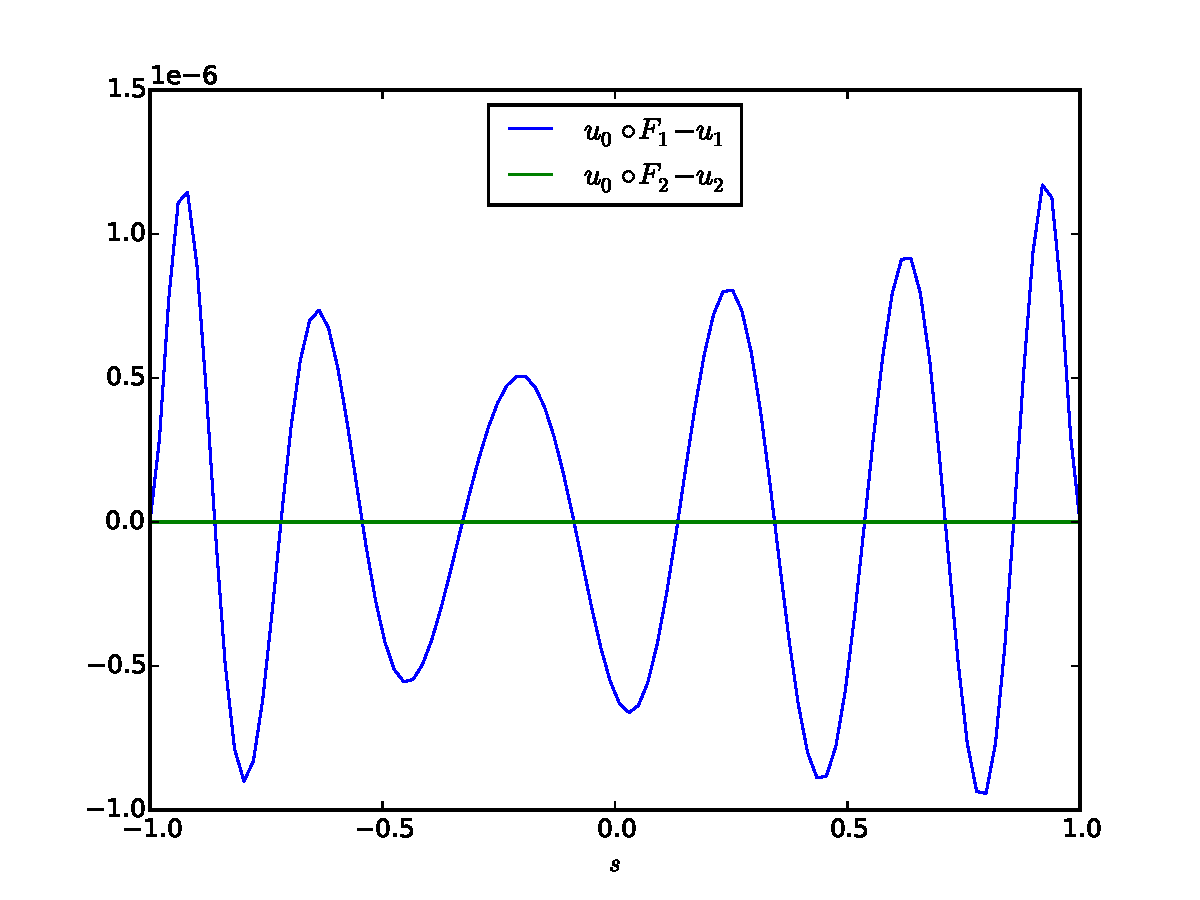
\includegraphics[width=0.45\textwidth]{img/shen_u0_ur}
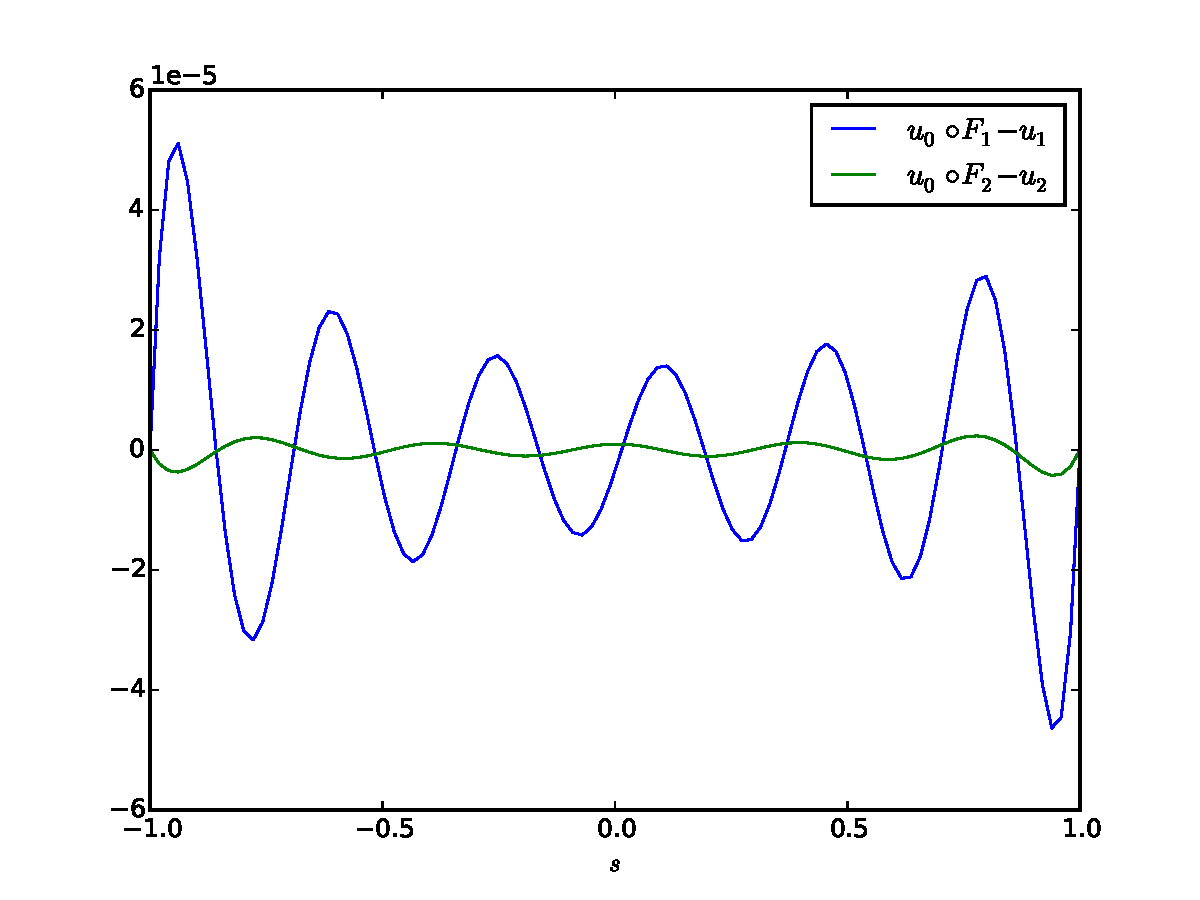
\includegraphics[width=0.45\textwidth]{img/sine_u0_ur}\\
\caption{
}
\label{fig:conds}
\end{figure}


\begin{figure}[ht]
\centering
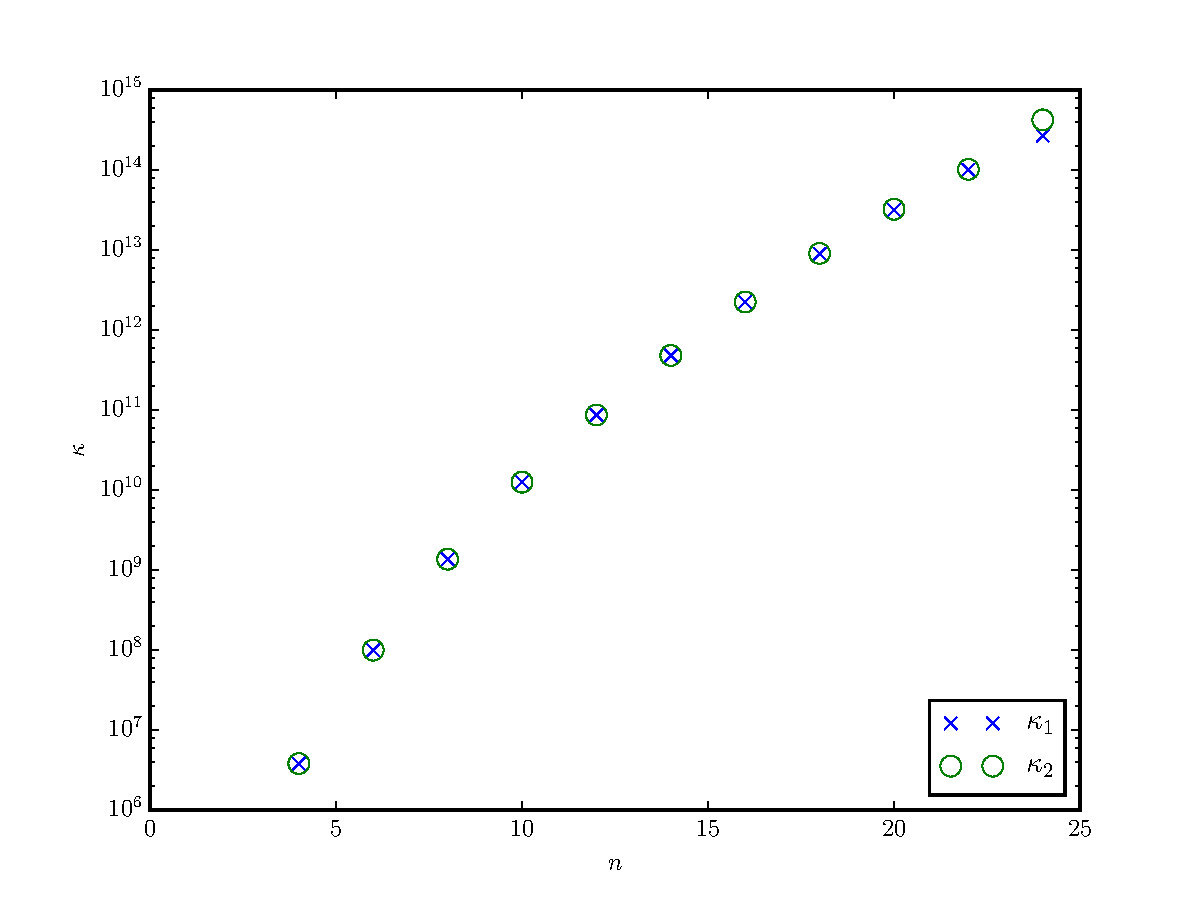
\includegraphics[width=0.45\textwidth]{img/shen_cond}
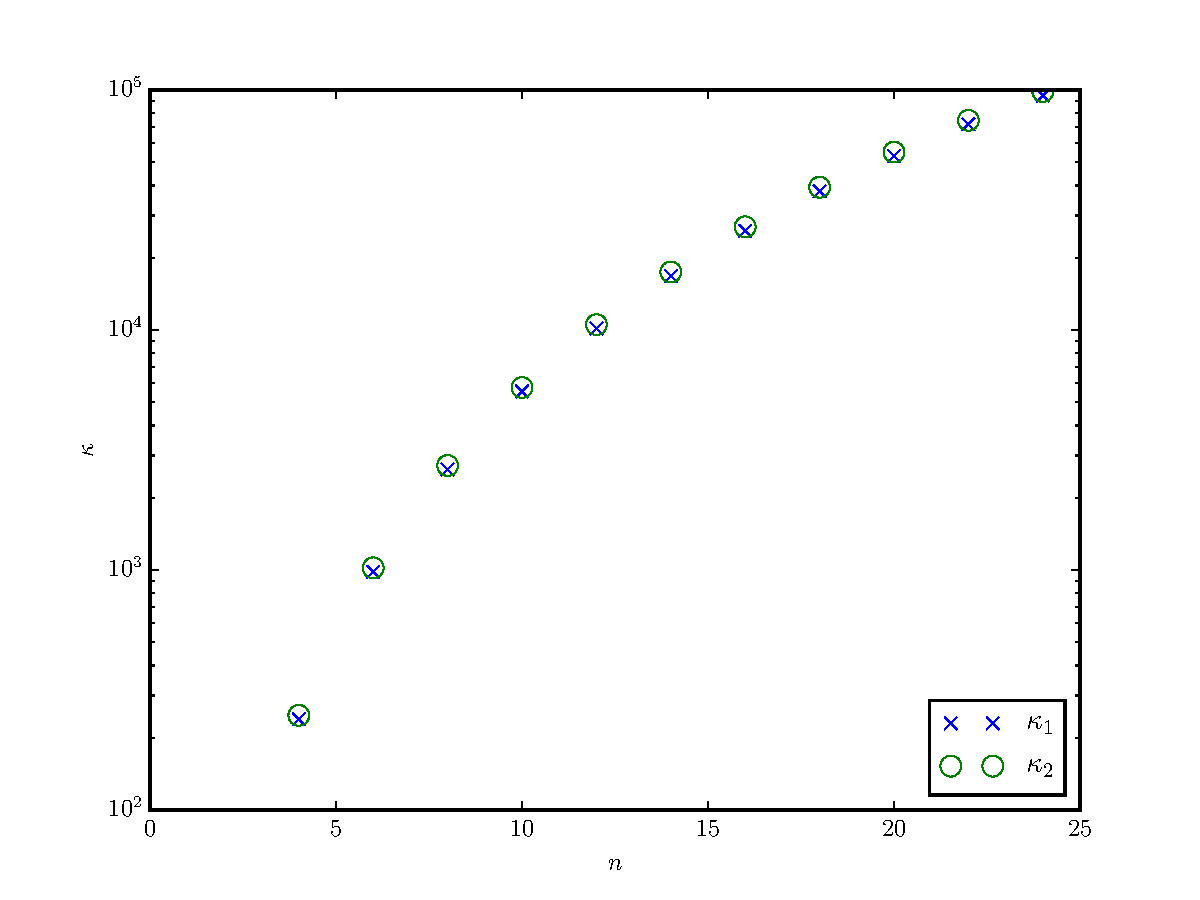
\includegraphics[width=0.45\textwidth]{img/sine_cond}\\
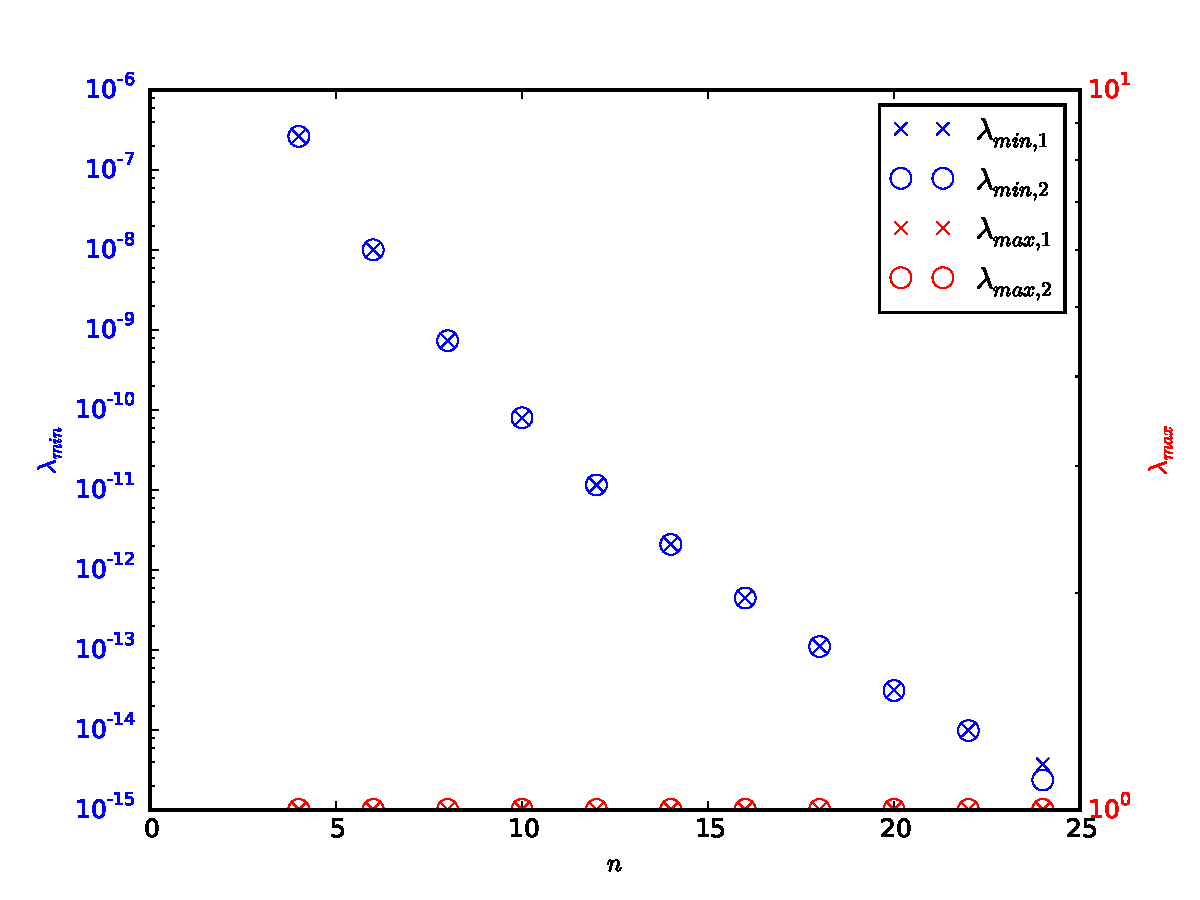
\includegraphics[width=0.45\textwidth]{img/shen_spectrum}
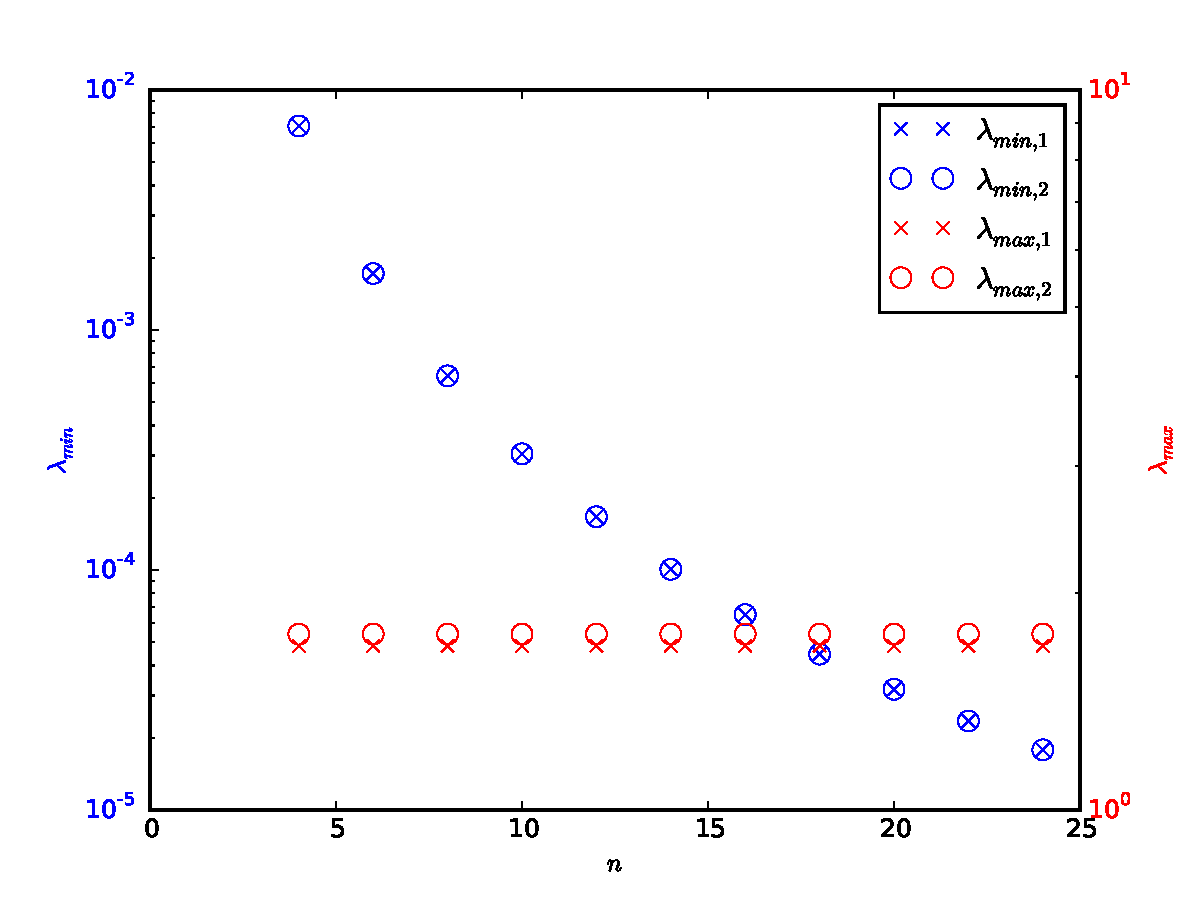
\includegraphics[width=0.45\textwidth]{img/sine_spectrum}\\
\caption{}
\label{fig:no_precon}
\end{figure}

\begin{figure}[ht]
\centering
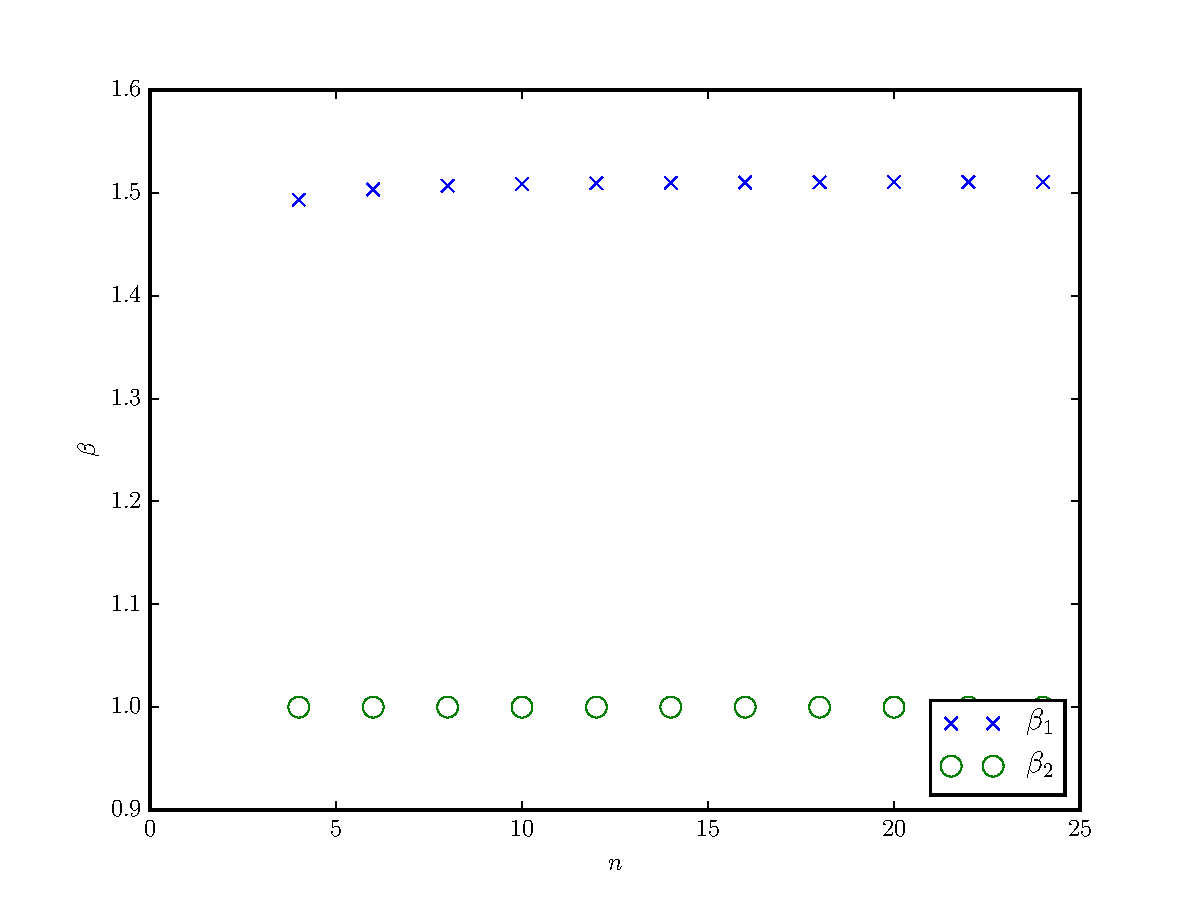
\includegraphics[width=0.45\textwidth]{img/Schur_precond_shen_cond}
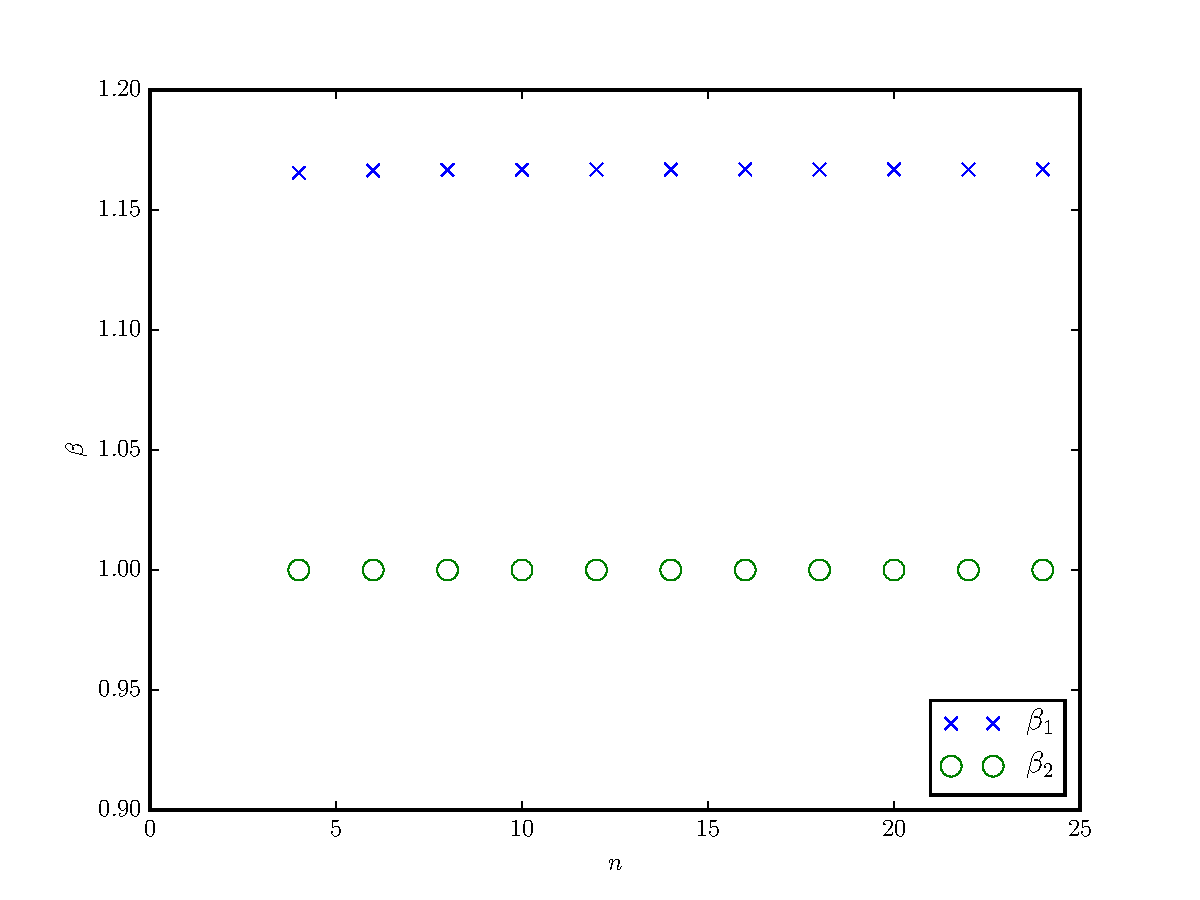
\includegraphics[width=0.45\textwidth]{img/Schur_precond_sine_cond}\\
\caption{}
\label{fig:Schur}
\end{figure}

\begin{figure}[ht]
\centering
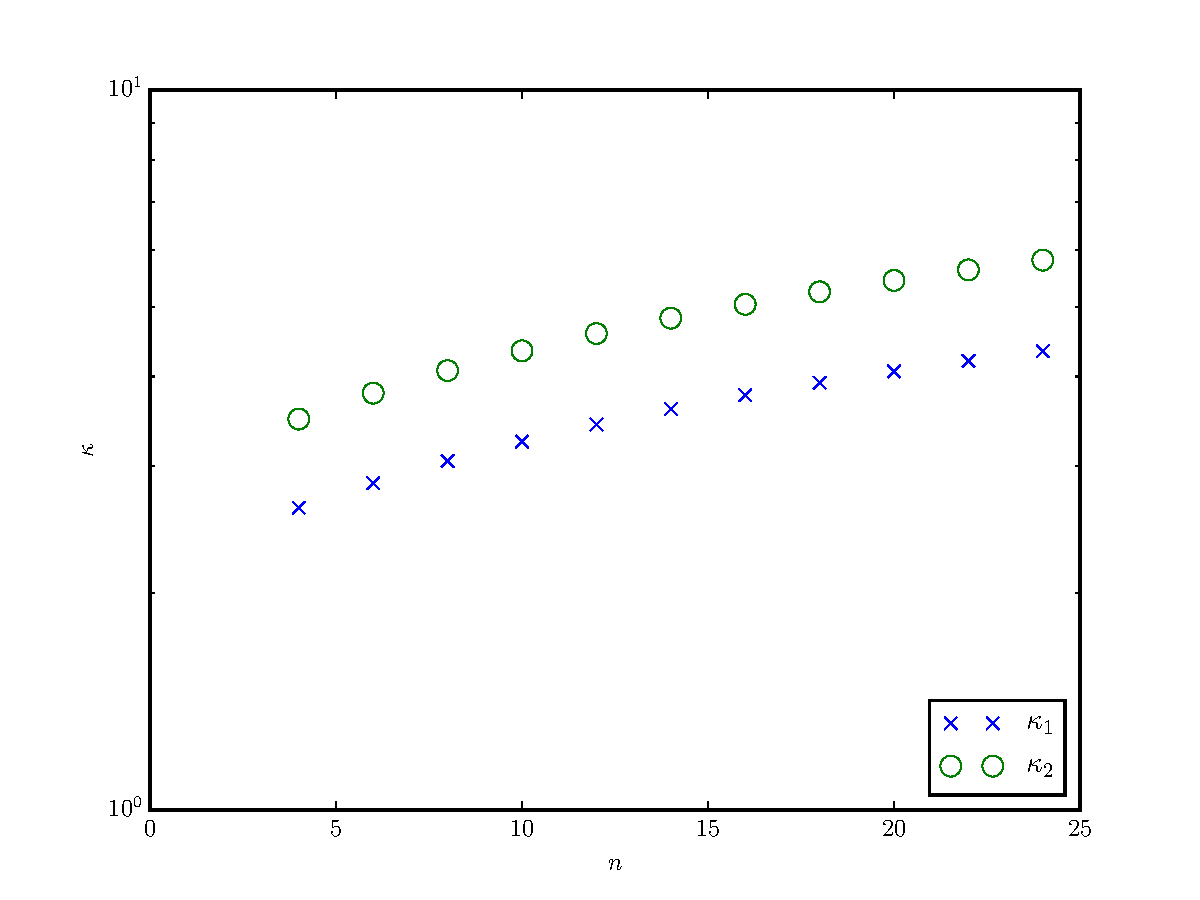
\includegraphics[width=0.45\textwidth]{img/precond_shen_cond}
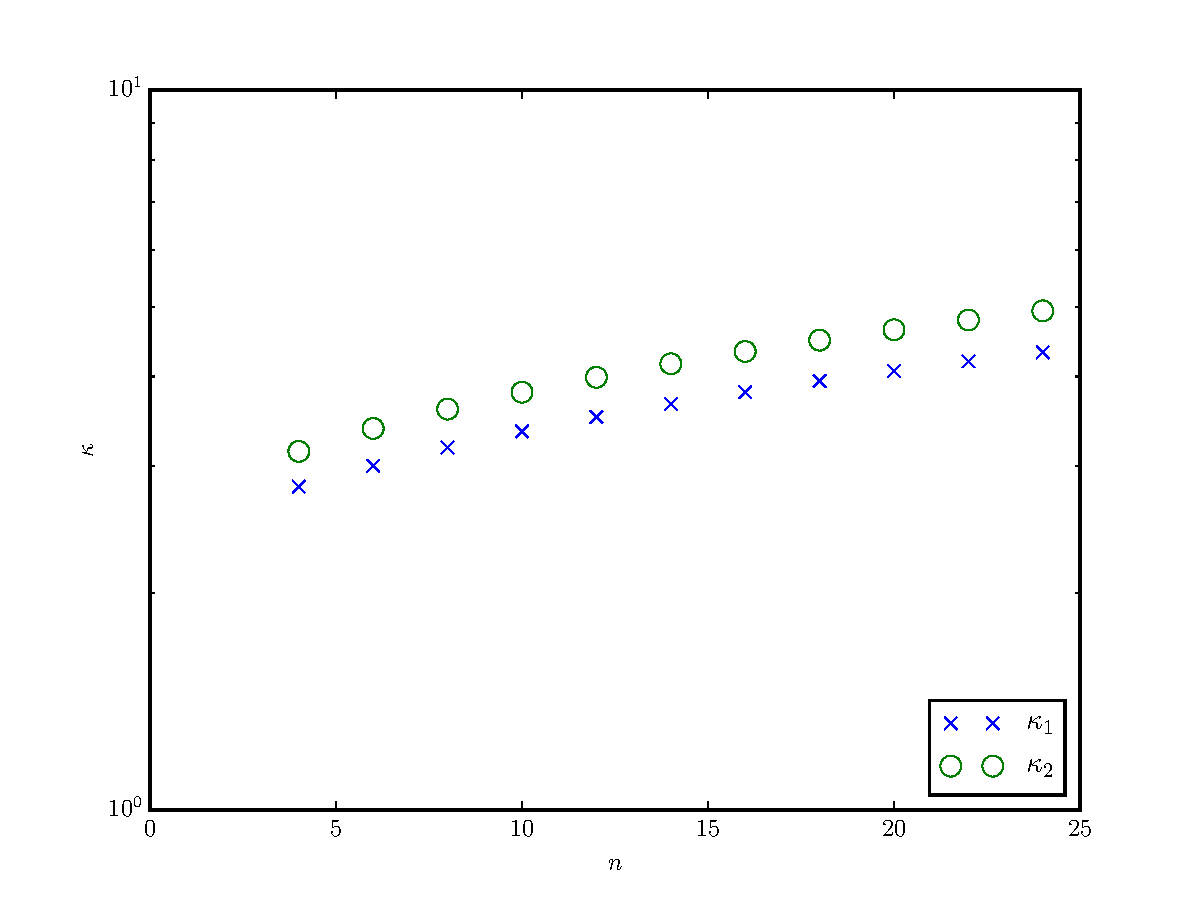
\includegraphics[width=0.45\textwidth]{img/precond_sine_cond}\\
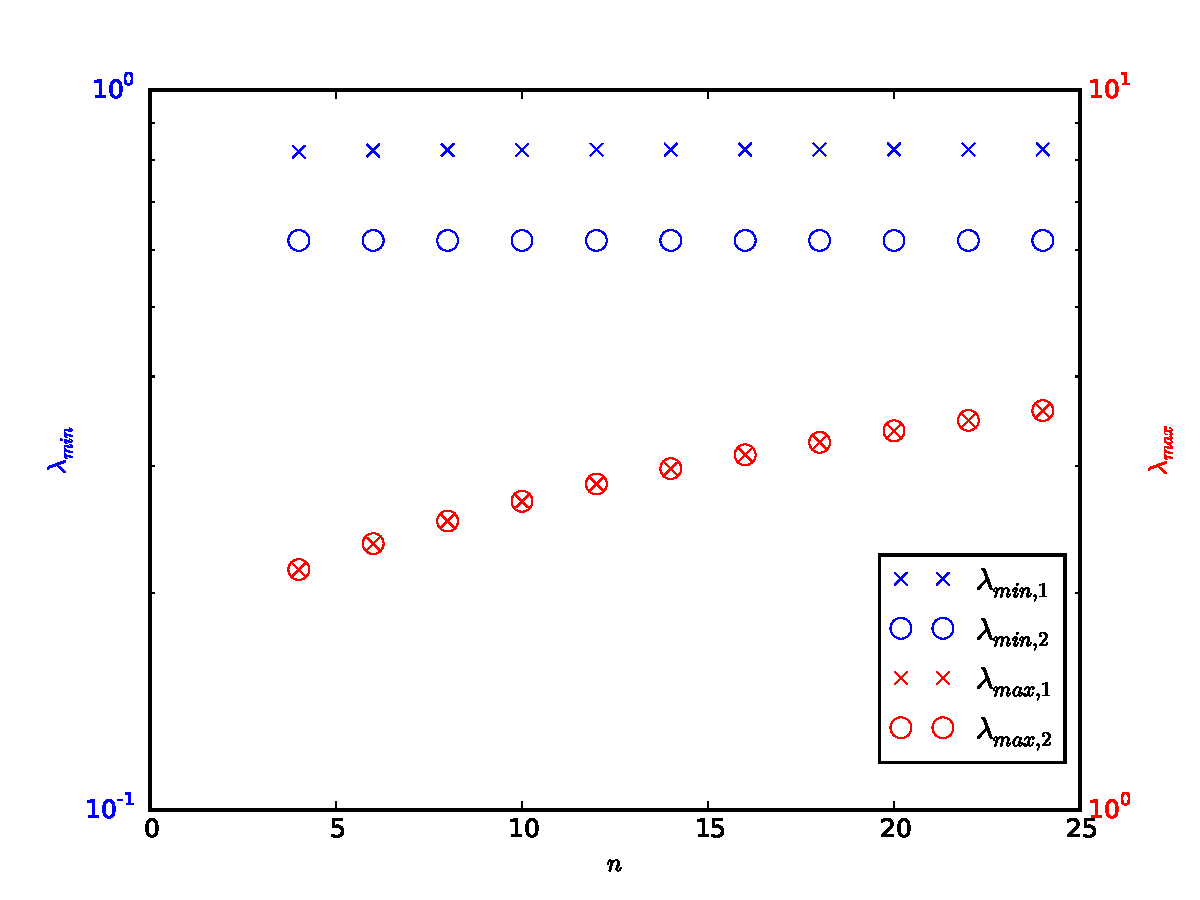
\includegraphics[width=0.45\textwidth]{img/precond_shen_spectrum}
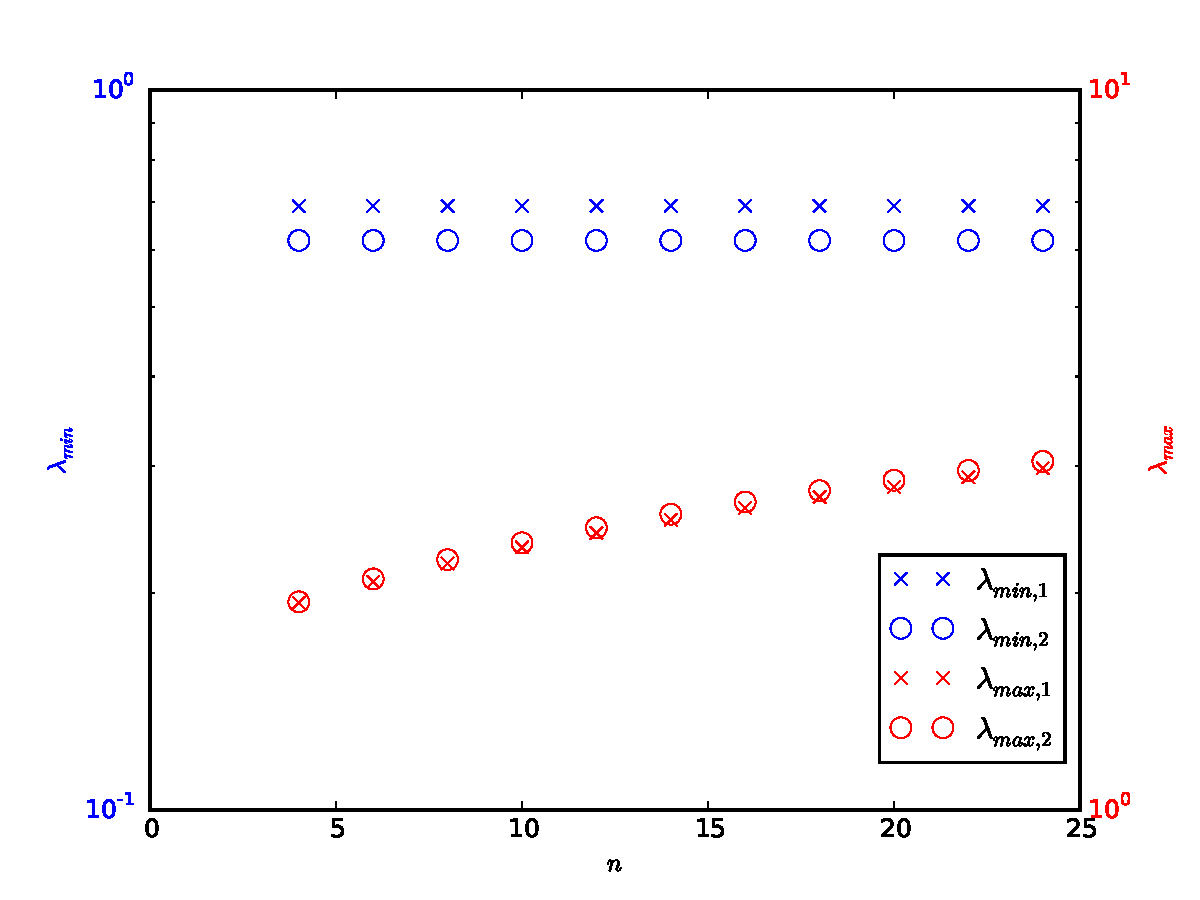
\includegraphics[width=0.45\textwidth]{img/precond_sine_spectrum}\\
\caption{}
\label{fig:precond}
\end{figure}

\section{Eigenvalues}
\label{sec:lbb}
When the basis are explained. We show kappa of both matrices as matrix
increases-preconditioner is needed for it locks (1beam 2 beams). The story has
to be that we are looking for the preconditioner but not find it yet. We focus
on the smallest eigenvalue of Schur. Simple configuration, ... . Maybe we can
do two beams and see how lmin effects. I think it is best to be honest. If we
try A, the cond increases for lmax, also we are not robust with respect to
material and beam position ... So this should be future work.

\section{Showcase}
Will not have rates but we can show same domain multiple beans different bcs. If
the nonlinearity is included.... If the precond works at least in one case solve
the problem iteratively.
% Preconditioning, uzawa, block lu

\section{Conclusions and extensions}
\label{sec:end}
Combine different families of functions...








Here we shall consider 
the plate as a simply connected rectangular domain


spanned 
either by the basis functions presented in \cite{shen} or 


Here we shall
consider


Here we shall consider domain 
$\Omega$ 
% global, sparse, spectral, framework components to solve (1) with only few
% changes, basis are presented, discuss LBB in both by eigenvalue problems,
% conclusies and future work


%    \sum_{r=1}^k\frac{E_r}{2}\int_{\mathcal{I}}\deriv{^2u_r}{s^2}\deriv{^2u_r}{s^2}J_r^{-3}+
%    \sum_{r=1}^k\int_{\mathcal{I}}\left(u_0\cdot F_r - u_r\right)\lambda_r J_r
%  -\displaystyle\int_{\Omega}f u_0.
%\]






On the other hand, Galerkin method with test spaces spanned by functions with 
global support is a natural choice for simply connected rectangular domains $\Omega$.



We shall in Section \ref{sec:abstract} 
% Lagrange 

Here we
shall consider test spaces spanned by the Legendre presented
based on functions with a global support are a natural choice. 

% For sufficiently smooth solution of (\ref{eq:foo}) the integration by parts yields
% that $u$ solves the system
% \begin{equation}
%   \label{eq:bar}
%   \begin{aligned}
%     E_0\Delta^2 u_0 &= f\text{ in }\Omega\\
%     E_r\deriv{^4 u_r}{s^4} &= 0 \text{ on }\mathcal{I}, r=1, 2,\cdots k\\
%     u_0 &= u_r \circ F^{-1}_r \text{ on }\Gamma_r
%   \end{aligned}
% \end{equation}
% subjected to the simply-supported boundary conditions
% \[
%   u\left(x\right) = \Delta u\left(x\right) = 0\quad x\in\partial\Omega\quad\text{and}\quad
%   u_r\left(s_i\right) = \deriv{^2 u_r}{s^2}\left(s_i\right)=0\quad i = 0, 1
% \]
% or the clamped boundary conditions
% \[
%   u\left(x\right) = \frac{\partial u}{\partial n}\left(x\right) = 0\quad x\in\partial\Omega\quad\text{and}\quad
%   u_r\left(s_i\right) = \deriv{u_r}{s}\left(s_i\right)=0\quad i = 0, 1.
% \]
% 
% With a general domain $\Omega$ the problem (\ref{eq:foo}) is arguably best solved 
% by splines or the finite element method. For the latter, special techniques are
% required to handle the fourth order operators in (\ref{eq:bar}). The problem can
% be discretized with 

Here On the other hand, the plate $\Omega$ is a simple domain


Due to biharmonic operator in (\ref{eq:bar}) the problem 

\newpage
\begin{thebibliography}{99}

\bibitem{reddy} Reddy B.D., \textit{Introductory functional analysis: with applications
  to boundary value problems and finite elements}, Springer, (1998).

%\bibitem{brezzi} Brezzi F., On the existence, uniqueness and approximation of saddle-point problems arising from Lagrangian multipliers,
%  \textit{Mathematical Modelling and Numerical Analysis-Mod{\'e}lisation Math{\'e}matique et Analyse Num{\'e}rique},
%  (1974), 
%  \textbf{8}: 129--151.
%
%\bibitem{brenner} Brenner S.C. and Scott R., \textit{The Mathematical Theory of Finite Element Methods},
%  Springer, (2008).
%
%\bibitem{babuska} Babu\v{s}ka I., The finite element method with Lagrangian
%  multipliers, \textit{Numerische Mathematik}, (1973), \textbf{20(3)}: 179--192.
%
%\bibitem{sympy} {{SymPy Development Team}},
%  \textit{SymPy: Python library for symbolic mathematics}, (2014),
%  http://www.sympy.org.
%
%\bibitem{shen} Shen, J., Efficient spectral-Galerkin method I. Direct solvers of
%  second-and fourth-order equations using Legendre polynomials, \textit{SIAM
%  Journal on Scientific Computing}, (1994), \textbf{15(6)}: 1489--1505.
%
  % \bibitem{numpy}
  %   @Misc{,
  %   author =    {Eric Jones and Travis Oliphant and Pearu Peterson and others},
  %   title =     {{SciPy}: Open source scientific tools for {Python}},
  %   year =      {2001--},
  %   url = "http://www.scipy.org/",
  %   note = {[Online; accessed 2015-05-03]}
  % }
  % 
  % \bibitem{cython}
  % Stefan Behnel, Robert Bradshaw, Craig Citro, Lisandro Dalcin, Dag Sverre Seljebotn and Kurt Smith. Cython: The Best of Both Worlds, Computing in Science and Engineering, 13, 31-39 (2011),
  % 
  % 
  % \bibitem{fenics}
  %   Logg A., Mardal K.-A., Wells G.N. et al.,
  %   \textit{Automated Solution of Differential Equations by the Finite Element Method},
  %   Springer, (2012).
  % 
  % \bibitem{swig}
  %   @inproceedings{Beazley:1996:SEU:1267498.1267513,
  %  author = {Beazley, David M.},
  %  title = {SWIG: An Easy to Use Tool for Integrating Scripting Languages with C and C++},
  %  booktitle = {Proceedings of the 4th Conference on USENIX Tcl/Tk Workshop, 1996 - Volume 4},
  %  series = {TCLTK'96},
  %  year = {1996},
  %  location = {Monterey, California},
  %  pages = {15--15},
  %  numpages = {1},
  %  url = {http://dl.acm.org/citation.cfm?id=1267498.1267513},
  %  acmid = {1267513},
  %  publisher = {USENIX Association},
  %  address = {Berkeley, CA, USA},
  % } 
  % 
  % \bibitem{oasis}
  % @article{mortensen2015oasis,
  %   title={Oasis: A high-level/high-performance open source Navier--Stokes solver},
  %   author={Mortensen, Mikael and Valen-Sendstad, Kristian},
  %   journal={Computer Physics Communications},
  %   volume={188},
  %   pages={177--188},
  %   year={2015},
  %   publisher={North-Holland}
  % }

\end{thebibliography}





\end{document}
=======
\documentclass{marine_2015}
     
\usepackage{graphicx}
\usepackage{amsmath}
\usepackage{amsfonts}
\usepackage{amssymb}

\newcommand{\Amat}{\ensuremath{\mathbb{A}}}
\newcommand{\Bmat}{\ensuremath{\mathbb{B}}}
\newcommand{\bvec}{\ensuremath{\mathbf{b}}}
\newcommand{\uvec}{\ensuremath{\mathbf{u}}}
\newcommand{\RM}{\ensuremath{RM}}
\newcommand{\inner}[2]{\ensuremath{\left(#1, #2\right)}}
\newcommand{\tuple}[2]{\ensuremath{\left[#1, #2\right]}}

\newcommand{\ainner}[2]{\ensuremath{a\left(#1, #2\right)}}
\newcommand{\binner}[2]{\ensuremath{b\left(#1, #2\right)}}
\newcommand{\Linner}[1]{\ensuremath{L\left(#1\right)}}
\newcommand{\Vh}{\ensuremath{V_{\mathbf{n}}}}
\newcommand{\Qh}{\ensuremath{Q_{\mathbf{m}}}}

\newcommand{\norm}[1]{\ensuremath{\left\|#1\right\|}}
\newcommand{\vvec}[1]{\ensuremath{\pmb{#1}}}
\newcommand{\deriv}[2]{\ensuremath{\frac{\mathrm{d}#1}{\mathrm{d}#2}}}
\newcommand{\tderiv}[2]{\ensuremath{\tfrac{\mathrm{d}#1}{\mathrm{d}#2}}}
\newcommand{\mm}[1]{({\bf mm comment:} \emph{#1})}

\title{
  BEND$\left|\text{P}\right|$Y: PYTHON FRAMEWORK FOR COMPUTING BENDING OF COMPLEX PLATE-BEAM SYSTEMS
}

\author{MIKAEL MORTENSEN$^{1, 2}$ AND MIROSLAV KUCHTA$^{1}$ AND KENT-ANDRE MARDAL$^{1, 2}$ }

\heading{Mikael Mortensen, Miroslav Kuchta and Kent-Andre Mardal}

\address{$^{1}$
Department of Mathematics, Division of Mechanics, University of Oslo,\\
0316 Oslo, Norway
  \and
$^{2}$ 
Center for Biomedical Computing, Simula Research Laboratory,\\
P.O. Box 134, No-134 Lysaker, Norway
}

\keywords{biharmonic equation, Lagrange multipliers, Schur complement}

\abstract{
We present a light-weight Python module for computing small deformations of a 
single plate supported by an arbitrary number of possibly intersecting
stiffeners. We show how the problem fits into the framework of abstract 
saddle point problems and how this abstraction can be exploited for clean design 
of the code. Stability properties of the resulting linear systems for two different 
sets of basis functions, namely, the eigenfunctions of the biharmonic operator 
and specialized Legendre polynomials are discussed. 
}

\begin{document}

\section{Introduction}
% What are we solving?
In this paper we discuss Galerkin methods for finding the equilibrium state of a 
physical system formed by a loaded thin plate and several beams that are constrained 
to deform together with the plate. Denoting $k$ the number of supporting beams, 
the equilibrium state is found as the solution of a constrained minimization problem
\begin{equation}
  \label{eq:foo}
  u = \min_{v\in V} \mathcal{E}\left(v\right)\quad\text{ and }\quad u_0\circ F_r
  = u_r, r=1, 2, \cdots k,
\end{equation}
where the energy functional $\mathcal{E}$ is defined as
\[
  \mathcal{E}\left(u\right)=
    \frac{E_0}{2}\displaystyle\int_{\Omega}\Delta u_0\,\Delta u_0+
    \sum_{r=1}^k\frac{E_r}{2}\int_{\mathcal{I}}
  \deriv{^2u_r}{s^2}\deriv{^2u_r}{s^2}J_r^{-3}
  -\displaystyle\int_{\Omega}f u_0.
\]
Here $V=V_0\times V_1 \times\cdots\times V_k$ is a function space with $k+1$
components. The first component $V_0$ contains functions that map the plate
domain $\Omega$ to real numbers and is therefore the space where the plate's
vertical displacement $u_0$ is found. The remaining components in $V$ contain the 
vertical displacements of individual beams $u_r$, i.e., the scalar 
functions whose domain is the interval $\mathcal{I}$. Moreover each beam is
considered as a set $\Gamma_r=\left\{x\in\Omega, x=F_r\left(s\right), s\in\mathcal{I}\right\}$
defined by an invertible mapping $F_r$ with Jacobian $J_r$. Note that for straight 
beams the Jacobian is simply the length of
the beam divided by the length of the interval. The mapping $F_r$ is also 
required to satisfy the conditions $F_r\left(s_0\right), F_r\left(s_1\right)\in\partial\Omega$ 
for $s_0, s_1$ the endpoints of $\mathcal{I}$. No beam is thus allowed to end inside 
the plate. Finally $f$ denotes the load while $E_0, E_r, r=1,2,\cdots k$ are 
constant parameters which, following the Kirchhoff-Love and Euler-Bernoulli
hypothesis (see, e.g., \cite{reddy}), depend on the material and geometry.

Introducing $k$ Lagrange multipliers $\lambda_k\in Q_k$, where the functions in 
$Q_k$ map the interval $\mathcal{I}$ to scalars, the constrained problem 
(\ref{eq:foo}) can be equivalently written as a search for extrema of the Lagrangian
$\mathcal{L}$,
\begin{equation}
  \label{eq:bar}
\mathcal{L}\left(u, \lambda\right) = \mathcal{E}\left(u\right) +
  \sum_{r=1}^k\int_{\mathcal{I}}\left(u_0\cdot F_r - u_r\right)\lambda_r J_r.
\end{equation}
The space $Q$ and function $\lambda\in Q$ are defined analogically as in (\ref{eq:foo}).
We note that the unconstrained problem (\ref{eq:bar}) is solvable only for
suitable pair of spaces $V, Q$ for which the requirements of the
Babu\v{s}ka-Brezzi\cite{babuska, brezzi} theory are satisfied.

% It can be solved with FEM but simple geometry ... global functions, spectral
% Galerkin
For a complex domain $\Omega$ the finite element method is arguably the most 
suitable method to solve the problem (\ref{eq:bar}). If, on the other hand, the
domain is simple, the Galerkin method with globally supported basis functions
can be applied. Note that the finite element method is an instance of the Galerkin 
method with test spaces spanned by the functions with local support. Regardless
of the basis functions employed, the stable discretization of (\ref{eq:bar})
requires that the Babu\v{s}ka-Brezzi conditions be satisfied by the constructed
finite dimensional spaces. We remark that in addition to stability
considerations the finite element discretization of the problem is also complicated
by the presence of the biharmonic operator, which requires techniques for fourth order 
problems (see e.g. \cite{brenner}). The approximations of $V$ must be constructed 
from $C^1$ continuous elements, e.g. Argyris element \cite{argyris}, or non-conforming 
elements, e.g. Morley element\cite{morley}. Alternatively, discontinuous elements with 
suitable stabilization \cite{brenner_ip} can be used. 

Here we shall consider the plate as a simply connected rectangular domain and as
such focus on Galerkin methods with test functions having global support.
Further, the two selected basis are designed for the fourth order problems and thus 
only the Babu\v{s}ka-Brezzi theory needs to be considered to derive a stable
discretization of problem (\ref{eq:bar}). The methods are discussed within a
framework for abstract saddle point problems reviewed in Section
\ref{sec:abstract}. The framework serves to identify the few common
elements(matrices) that are required to easily introduce Galerkin discretizations of
(\ref{eq:bar}) based on any set of basis functions. Properties of the two sets of
basis functions considered in this paper are then compared in Section \ref{sec:basis}.
Finally in Section \ref{sec:lbb} the inf-sup condition for the two proposed
disretizations is discussed.

\section{Abstract framework for saddle point problems}
\label{sec:abstract}
% conditions for extrema
The necessary conditions for the extreme point of the Lagrangian $\mathcal{L}$
from (\ref{eq:bar}) define $2k+1$ equations to be satisfied by the $2k+1$
unknowns $\left(u, \lambda\right)\in V\times Q$. These equations read
\[
  \begin{aligned}
    \label{eq:system}
    E_0\displaystyle\int_{\Omega}\Delta u_0\,\Delta v_0-
    \sum_{r=1}^k\int_{\mathcal{I}}v_0\lambda_r J_r &=\displaystyle\int_{\Omega}f
    v_0\quad\forall v_0\in V_0,& \\
    E_r\displaystyle\int_{\mathcal{I}}
    \deriv{^2u_r}{s^2}\deriv{^2v_r}{s^2}J_r^{-3} +
  \int_{\mathcal{I}} u_r \lambda_r J_r &= 0\quad\forall v_r\in V_r, r=1,
    2\cdots, k,&\\
  \int_{\mathcal{I}}\left(u_r-u_0\right)\mu_r J_r &= 0\quad\forall \mu_r\in Q_r,
    r=1, 2\cdots, k&.\\
  \end{aligned}
\]
To apply the Babu\v{s}ka-Brezzi theory of abstract saddle point problems to (\ref{eq:system})
the system is rewritten in terms of bilinear forms $a:V\times V\mapsto \mathbb{R}$, $b:Q\times V\mapsto \mathbb{R}$
and a linear form $L:V\mapsto R$. Here 
$\ainner{u}{v}=\sum_{r=0}^{k}\ainner{u_r}{v_r}_r$ where \mm{Missing text}




% how the problem fits saddle
% Galerkin and how A, B are formed for r. The elements that are needed for
% efficiency: mass, stiffness, bending, (fast inner product). Probably mention sparsity
% Eigenvalue problem for LBB.





Let $\mathcal{I}$ denote a nonempty interval. As we are in the following
interested in domains that have a Cartesian product structure we consider without
loss of generality $\Omega=\mathcal{I}\times\mathcal{I}$. We shall refer to this
domain as \textit{plate}. Further let $w_i, i=1, 2,\cdots, k$ be a set of curves 
$w_i=\left\{\vec{x}\in\Omega, \vec{x}=\vec{F}_i\left(s\right),
s\in\mathcal{I}\right\}$, where $\vec{F_i}$ is a smooth invertible mapping with
Jacobian $J_i>0$ that additionally satisfies $\vec{F}_i\left(s_0\right),
\vec{F}_i\left(s_1\right)\in\partial\Omega$ and
$\vec{F}_i\left(s_0\right) \neq \vec{F}_i\left(s_1\right)$ for $s_0, s_1$ the
endpoints of interval $\mathcal{I}$. These curves, and occasionally the
respected mappings are referred to as \textit{beams}. In this paper we are for the
most part concerned with straight/linear beams, that is, we consider mappings
$\vec{F}_i\left(s\right)=\vec{P}_i\tfrac{s_1-s}{s_1-s_0}+\vec{Q}_i\tfrac{s_0-s}{s_0-s_1}$
determined by pairs of mutually distinct points $\vec{P}_i, \vec{Q}_i$ that
are located on the boundary of the plate. \mm{Use that over which when the added sentence puts a restriction on the objects it refers to. E.g. dogs that are pink, not dogs which are pink.} Note that in this case
$J_i=\tfrac{\left|\vec{P}_i-\vec{Q}_i\right|}{2}$. 
% you do linear so absorb jacobian into material!!! KISS
%
%
%
With these assumptions on geometry we let $V, \hat{V}_i, i=1, 2, \cdots, k$ denote
spaces of functions that map respectively the plate and the beams to real
numbers. By invertibility of $\vec{F}_i$ each function space $\hat{V}_i$ can be
associated with a function space $V_{i}$ that maps the reference interval
$\mathcal{I}$ to real numbers. Indeed for $v\in V_i$ function
$\hat{v}=v\circ\vec{F}_i$ belongs to $\hat{V}_i$.

Let $u\in V, u_i\in V_i, i=1, 2, \cdots, k$ and consider the problem of
minimizing the Lagrangian
\[
  \mathcal{L}\left(u, u_1, u_2, \cdots, u_k\right)=
  \frac{E}{2}\displaystyle\int_{\Omega}\Delta u\,\Delta u+
  \sum_i\frac{E_i}{2}\int_{\mathcal{I}}
  \deriv{^2u_i}{s^2}\deriv{^2u_i}{s^2}J_i^{-3}
  -\displaystyle\int_{\Omega}f u
\]
subjected to $k$ constraints
$T(u)=u_i$, here $T(u)$ is a short hand for the composition of trace and the
pullback inverse.\textit{explain the constraint, trace, Sobolev?}.
We build the constraint into the Lagrangian. To this end consider spaces $Q_i$
and functions (Lagrange multipliers) $\lambda_i\in Q_i$. Moreover let
$Q=Q_0\times Q_1\times\cdots\times Q_k$ and $\vvec{\lambda}\in
Q,\vvec{\lambda}_i=\lambda_i$ \mm{???} and a problem
\[
  \mathcal{L}\left(u, u_1, u_2, \cdots, u_k;\vvec{\lambda}\right)=
   \frac{E}{2}\displaystyle\int_{\Omega}\Delta u\,\Delta u+
  \sum_i\frac{E_i}{2}\int_{\mathcal{I}}
  \deriv{^2u_i}{s^2}\deriv{^2u_i}{s^2}J_i^{-3}
  -\displaystyle\int_{\Omega}f u - \sum_i\int_{\mathcal{I}}\left(u-u_i\right)\lambda_i J_i
\]
The necessary condition for extrema are then
Under additional regularity we can make Euler Lagrange equations \mm{rewrite}
\[
  \begin{aligned}
    E\Delta^2u &= f\quad\text{ in }\Omega\\
    E_i\deriv{^4 u_i}{s^4} &= 0\quad\text{ on }\mathcal{I}\\
    u &= u_i\quad\text{ on }\mathcal{I}\\
  \end{aligned}
\]
subjected to boundary conditions $u=0, \partial_nu=0$ and $u_i=0, \tderiv{u_i}{s}=0$
$u=0, \Delta u=0$ and $u_i=0, \tderiv{^2u_i}{s^2}=0$. \textit{What are these called?}
Abstract saddle $V:=V\times V_1, \times V_2, \cdots, \times V_k$,
$V\ni\vvec{u}=\left(u, u_1, u_2, \cdots, u_k\right)$ and define bilinear form
$a:V\times V\mapsto\mathbb{R}$ as \mm{missing $v$ below:}
\[
  \ainner{\vvec{u}}{\vvec{v}} = 
  E\displaystyle\int_{\Omega}\Delta u\,\Delta+
  \sum_iE_i\displaystyle\int_{\mathcal{I}} \deriv{^2u_i}{s^2}\deriv{^2v_i}{s^2}J_i^3
\]
$b:V\times Q\mapsto\mathbb{R}$ as
\[
  \binner{\vvec{v}}{\vvec{\lambda}} = 
  \int_{\mathcal{I}}\left(v_i-v\right)\lambda_i J_i
\]
Finally linear form
$L:V\mapsto\mathbb{R}$ as
\[
  \displaystyle\int_{\Omega}f v
\]
%FIXME it is much better to use V_0 and then V...
% Saddle
Then the problem becomes simply: Find $\vvec{u}\in V, \vvec{\lambda}\in Q$ such
that $\ainner{u}{v}+\binner{v}{\lambda}+\binner{u}{\mu}=\Linner{v}$ for all 
$\vvec{v}\in V, \vvec{\mu}\in Q$. You have babuska theory that gives you
continuous existence. Don't go there... Discrete mention Stokes taylor hood, or
the compatibility condition from spectral.
% Galerkin
The finite dimensional approximation of $V$ is $\Vh$. Here $\mathbf{n}$ is a
multiindex of length $k+1$ and $\mathbf{n}_i, i=0, 1,\cdots, k$ denotes dimension
of the $i$-th component of $\Vh$ which is spanned by functions $\phi^i_j,
i=1,2,\cdots\mathbf{n}_i$. Note that $\phi^0_j$ are defined over $\Omega$ while
the rest have the reference interval as their domain. Similarly, we denote $\Qh$ 
the finite dimensional approximation of $Q$ is . Here $\mathbf{m}$ is a multiindex
of length $k$ and $\mathbf{m}_i, i=1, 2, \cdots, k$ denotes dimension of the 
$i$-th component of $\Qh$ spanned by functions $\psi^i_j, j=1,
2\cdots,\mathbf{m}_i$.
% Matrices
Let $n, m$ be respectively the sizes of multiindices $\mathbf{n}, \mathbf{m}$.
The abstract saddle point problem considered on the discerete subspaces
translates into the linear system: Find $\mathbf{U}\in\mathbb{R}^n,
\mathbf{P}\in\mathbb{R}^m$ such that
\[
    \begin{bmatrix}
      \mathbb{A} & \mathbb{B} \\
      \mathbb{B}^{\text{T}} & 0
    \end{bmatrix}
    \,
    \begin{bmatrix}
      \mathbf{U} \\
      \mathbf{P}
    \end{bmatrix}
    =
    \begin{bmatrix}
      \mathbf{b}\\
      0
    \end{bmatrix}.
\]
$\mathbf{b}\in\mathbb{R}^n$ has most entries zero except the first $\mathbf{n}_0$
entries which take the value $\inner{\phi^0_j}{f}$. The matrix
$\Amat\in\mathbb{R}^{n\times n}$ is block diagonal consisting of $k+1$
submatrices
\[
    \mathbb{A}=
    \begin{bmatrix}
      \mathbb{A}^0  &   &  &\\
                    & \mathbb{A}^1 &  &\\
                    &   &   \ddots    & \\
                    &   &   & \mathbb{A}^k\\
    \end{bmatrix}
\]
with $\mathbb{A}^0_{i, j}=E\inner{\Delta \phi^0_i}{\Delta\phi^0_j}$ and
$\mathbb{A}^r_{i, j}=E_r\displaystyle\int_{\mathcal{I}}
\deriv{^2\phi^r_i}{s^2}\deriv{^2\phi^r_j}{s^2}J_r^3$. Matrix
$\Bmat\in\mathbb{R}^{n\times m}$
\[
    \mathbb{B}=
    \begin{bmatrix}
      \mathbb{C}^1 & \mathbb{C}^2 & \cdots & \cdots & \mathbb{C}^k\\
      \mathbb{M}^1   &        0       & \cdots & \cdots &        0      \\
           0         & \mathbb{M}^2   &    0   & \cdots &   \vdots      \\
         \vdots      &       0        & \ddots & \ddots &   \vdots      \\
         \vdots      &     \vdots      & \ddots & \ddots &       0      \\
      0         &  \cdots        & \cdots & 0      &   \mathbb{M}^k     \\
    \end{bmatrix}
\]
where $\mathbb{C}^r_{ij}=\int_{\mathcal{I}}\phi^0_j\psi^r_i$ and
$\mathbb{M}^r_{ij}=\int_{\mathcal{I}}\phi^r_j\psi^r_i$, so the latter defines
a mass matrix between spaces.
Eigenvalue problems for wellposedness/stability. Programming needs assembler
so just take into accont the multiindex to get the position and size of the
block. What are blocks: we have mass matrix and the 1d 2d bending matrices.
Simplifies if $\phi^i=\psi^i$.

% Discussion on properties of basis. Some speedup with FFT
\section{Basis}
\label{sec:basis}
% For each basis how it is defined. How does A look, convergence properties for
% biharmonic problem(What happens if discontinuity). How does A scale. Comment
% on fast assembly
\subsection{Shen basis}
Described in shen. Legendre polynomials - we use for clamped boundary
conditions. Confirm spectral convergence in 1d and 2d. In 1d the biharmonic is
diagonal hence Ak matrices. But A0 is ... . Mass matrix is penta diagonal. How
does 2d bending matrix scale. Probably mention the tensor product. Mention
forward legendre transform.
\subsection{Eigen basis}
Consider eigenvalue problem. Find functions - spectral decomposition. Action of
Galerkin method with the basis. Convergence 1d, 2d. Matrices. Solution. If you
have time it would be really nice to solve 1d solution with rhs that has
different smoothness so that we see how it effects the rate in both cases.

\section{Eigenvalues}
\label{sec:lbb}
When the basis are explained. We show kappa of both matrices as matrix
increases-preconditioner is needed for it locks (1beam 2 beams). The story has
to be that we are looking for the preconditioner but not find it yet. We focus
on the smallest eigenvalue of Schur. Simple configuration, ... . Maybe we can
do two beams and see how lmin effects. I think it is best to be honest. If we
try A, the cond increases for lmax, also we are not robust with respect to
material and beam position ... So this should be future work.

\section{Showcase}
Will not have rates but we can show same domain multiple beans different bcs. If
the nonlinearity is included.... If the precond works at least in one case solve
the problem iteratively.
% Preconditioning, uzawa, block lu

\section{Conclusions and extensions}
\label{sec:end}
Combine different families of functions...








Here we shall consider 
the plate as a simply connected rectangular domain


spanned 
either by the basis functions presented in \cite{shen} or 


Here we shall
consider


Here we shall consider domain 
$\Omega$ 
% global, sparse, spectral, framework components to solve (1) with only few
% changes, basis are presented, discuss LBB in both by eigenvalue problems,
% conclusies and future work


%    \sum_{r=1}^k\frac{E_r}{2}\int_{\mathcal{I}}\deriv{^2u_r}{s^2}\deriv{^2u_r}{s^2}J_r^{-3}+
%    \sum_{r=1}^k\int_{\mathcal{I}}\left(u_0\cdot F_r - u_r\right)\lambda_r J_r
%  -\displaystyle\int_{\Omega}f u_0.
%\]






On the other hand, Galerkin method with test spaces spanned by functions with 
global support is a natural choice for simply connected rectangular domains $\Omega$.



We shall in Section \ref{sec:abstract} 
% Lagrange 

Here we
shall consider test spaces spanned by the Legendre presented
based on functions with a global support are a natural choice. 

% For sufficiently smooth solution of (\ref{eq:foo}) the integration by parts yields
% that $u$ solves the system
% \begin{equation}
%   \label{eq:bar}
%   \begin{aligned}
%     E_0\Delta^2 u_0 &= f\text{ in }\Omega\\
%     E_r\deriv{^4 u_r}{s^4} &= 0 \text{ on }\mathcal{I}, r=1, 2,\cdots k\\
%     u_0 &= u_r \circ F^{-1}_r \text{ on }\Gamma_r
%   \end{aligned}
% \end{equation}
% subjected to the simply-supported boundary conditions
% \[
%   u\left(x\right) = \Delta u\left(x\right) = 0\quad x\in\partial\Omega\quad\text{and}\quad
%   u_r\left(s_i\right) = \deriv{^2 u_r}{s^2}\left(s_i\right)=0\quad i = 0, 1
% \]
% or the clamped boundary conditions
% \[
%   u\left(x\right) = \frac{\partial u}{\partial n}\left(x\right) = 0\quad x\in\partial\Omega\quad\text{and}\quad
%   u_r\left(s_i\right) = \deriv{u_r}{s}\left(s_i\right)=0\quad i = 0, 1.
% \]
% 
% With a general domain $\Omega$ the problem (\ref{eq:foo}) is arguably best solved 
% by splines or the finite element method. For the latter, special techniques are
% required to handle the fourth order operators in (\ref{eq:bar}). The problem can
% be discretized with 

Here On the other hand, the plate $\Omega$ is a simple domain


Due to biharmonic operator in (\ref{eq:bar}) the problem 

\newpage
\begin{thebibliography}{99}

\bibitem{reddy} Reddy B.D., \textit{Introductory functional analysis: with applications
  to boundary value problems and finite elements}, Springer, (1998).

%\bibitem{brezzi} Brezzi F., On the existence, uniqueness and approximation of saddle-point problems arising from Lagrangian multipliers,
%  \textit{Mathematical Modelling and Numerical Analysis-Mod{\'e}lisation Math{\'e}matique et Analyse Num{\'e}rique},
%  (1974), 
%  \textbf{8}: 129--151.
%
%\bibitem{brenner} Brenner S.C. and Scott R., \textit{The Mathematical Theory of Finite Element Methods},
%  Springer, (2008).
%
%\bibitem{babuska} Babu\v{s}ka I., The finite element method with Lagrangian
%  multipliers, \textit{Numerische Mathematik}, (1973), \textbf{20(3)}: 179--192.
%
%\bibitem{sympy} {{SymPy Development Team}},
%  \textit{SymPy: Python library for symbolic mathematics}, (2014),
%  http://www.sympy.org.
%
%\bibitem{shen} Shen, J., Efficient spectral-Galerkin method I. Direct solvers of
%  second-and fourth-order equations using Legendre polynomials, \textit{SIAM
%  Journal on Scientific Computing}, (1994), \textbf{15(6)}: 1489--1505.
%
  % \bibitem{numpy}
  %   @Misc{,
  %   author =    {Eric Jones and Travis Oliphant and Pearu Peterson and others},
  %   title =     {{SciPy}: Open source scientific tools for {Python}},
  %   year =      {2001--},
  %   url = "http://www.scipy.org/",
  %   note = {[Online; accessed 2015-05-03]}
  % }
  % 
  % \bibitem{cython}
  % Stefan Behnel, Robert Bradshaw, Craig Citro, Lisandro Dalcin, Dag Sverre Seljebotn and Kurt Smith. Cython: The Best of Both Worlds, Computing in Science and Engineering, 13, 31-39 (2011),
  % 
  % 
  % \bibitem{fenics}
  %   Logg A., Mardal K.-A., Wells G.N. et al.,
  %   \textit{Automated Solution of Differential Equations by the Finite Element Method},
  %   Springer, (2012).
  % 
  % \bibitem{swig}
  %   @inproceedings{Beazley:1996:SEU:1267498.1267513,
  %  author = {Beazley, David M.},
  %  title = {SWIG: An Easy to Use Tool for Integrating Scripting Languages with C and C++},
  %  booktitle = {Proceedings of the 4th Conference on USENIX Tcl/Tk Workshop, 1996 - Volume 4},
  %  series = {TCLTK'96},
  %  year = {1996},
  %  location = {Monterey, California},
  %  pages = {15--15},
  %  numpages = {1},
  %  url = {http://dl.acm.org/citation.cfm?id=1267498.1267513},
  %  acmid = {1267513},
  %  publisher = {USENIX Association},
  %  address = {Berkeley, CA, USA},
  % } 
  % 
  % \bibitem{oasis}
  % @article{mortensen2015oasis,
  %   title={Oasis: A high-level/high-performance open source Navier--Stokes solver},
  %   author={Mortensen, Mikael and Valen-Sendstad, Kristian},
  %   journal={Computer Physics Communications},
  %   volume={188},
  %   pages={177--188},
  %   year={2015},
  %   publisher={North-Holland}
  % }

\end{thebibliography}


\end{document}
